\documentclass{beamer}
\usepackage[utf8]{inputenc}
\usepackage{fourier}

\usepackage{amsfonts}
\usepackage{amsmath}		
\usepackage{amssymb}
\usepackage{beamerthemesplit}
\usepackage{bezier}
\usepackage{float}
\usepackage{hyperref}
\usepackage{longtable}
\usepackage{makeidx}
\usepackage{rotating}
\usepackage{wrapfig}
\usepackage{multirow}
\usepackage{pgf}
\usepackage{ragged2e}

\usetheme{Madrid}
\usefonttheme{serif}
\usecolortheme{default}

\title[Graph Neural Networks]{Graph Neural Networks \\ Efficient Tensor Operations In CUDA/GPU \\ Custom Deep Learning Framework In C++ \\ Applications In Quantum Chemistry}
\author[Hy et al.]{Hy Truong Son, Chris Jones \\ Advisor: Prof. Risi Kondor}
\institute[UChicago]{The University of Chicago}
\date{December 2017}

\begin{document}

\logo{
\includegraphics[height=0.5cm]{Logo.jpg}}

\frame{\titlepage}

\begin{frame}
\frametitle{Table of Contents}
\tableofcontents
\end{frame}

\section{Chapter I: Introduction}

\begin{frame}
\frametitle{Our publication}
Covariant Compositional Networks For Learning Graphs (submitted to ICLR 2018)
\end{frame}

\begin{frame}
\frametitle{What are Graph Neural Networks?}
\begin{block}{Learning images, texts}
In general, traditional neural networks (Convolutional Neural Networks, Recurrent Neural Networks, etc.) take inputs as \textbf{fixed-size} vectors, matrices and tensors. The architecture of the neural network is always \textbf{fixed}.
\end{block}
\begin{alertblock}{Learning graphs, molecules}
A graph neural network is a neural network that takes inputs on graphs with \textbf{various} sizes and structures. The architecture of the neural network is always \textbf{dynamic}.
\end{alertblock}
\end{frame}

\begin{frame}
\frametitle{What are Tensor Operations?}
Basic tensors:
\begin{itemize}
	\item 1D Tensor: Vectors
	\item 2D Tensor: Matrices
	\item 3D Tensor: Cubes
\end{itemize}
What we are dealing with: {\color{red} 6D Tensors}. We need the \textbf{tensor contraction} operation $C$ to reduce from the \textbf{high-order} into a \textbf{low-order}:
$$C: \mathbb{R}^{d \times d \times d \times d \times d \times c} \rightarrow \mathbb{R}^{d \times d \times c}$$
\end{frame}

\begin{frame}
\frametitle{What is the GraphFlow framework?}
We wrote our own Deep Learning framework named {\color{red} GraphFlow} in C++ and CUDA to construct arbitrary neural networks supporing symbolic differentiation and dynamic computation graphs. 
\begin{itemize}
	\item Number of lines of C++ code: $\sim 55,000$
%	\item Total (including generated codes): $\sim 274,000$
	\item Number of lines written this quarter for parallelization: {\color{red} $\sim 10,000$}
\end{itemize}
\end{frame}

\begin{frame}
\frametitle{Why not use TensorFlow or PyTorch?}
\begin{block}{TensorFlow's disadvantage}
No (direct) support for dynamic computation graphs.
\end{block}
\begin{block}{PyTorch's disadvantage}
No support for tensor contractions.
\end{block}
\begin{alertblock}{GraphFlow's advantage}
	\begin{itemize}
		\item Support dynamic computation graphs
		\item Support tensor contractions
	\end{itemize}
\end{alertblock}
\end{frame}

\begin{frame}
\frametitle{Molecular Chemical Representation}
\begin{justify}
\begin{center}
	Harvard Clean Energy Project (HCEP) Dataset \cite{Johannes}
\end{center}
\begin{center}
	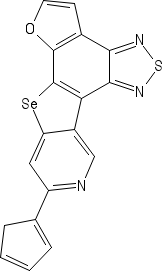
\includegraphics[scale=0.5]{sketcher}
\end{center}
Compound: C18H9N3OSSe \\
SMILES: C1C=CC=C1c1cc2[Se]c3c4occc4c4nsnc4c3c2cn1 \\
Power Conversion Efficiency (PCE, range 0 - 11): 5.16195
\end{justify}
\end{frame}

\begin{frame}
\frametitle{Molecular Graph Representation}
\begin{justify}
\begin{center}
	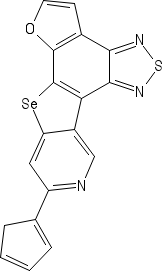
\includegraphics[scale=0.5]{sketcher}
	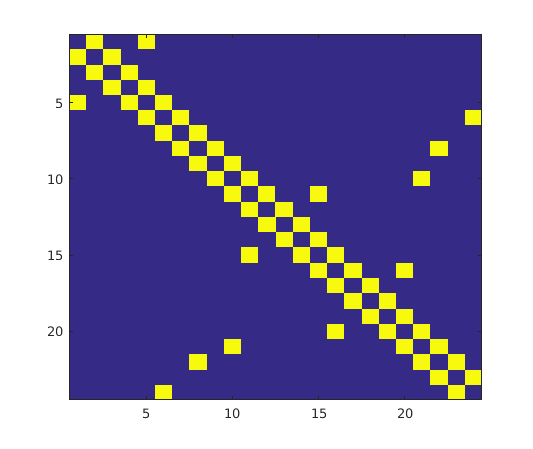
\includegraphics[scale=0.5]{adjacency}
\end{center}
C18H9N3OSSe \ \ \ \ \ \ \ \ \ \ \ \ \ \ \ \ \ \ \ \ Adjacency matrix
\end{justify}
\end{frame}

\section{Chapter II: State-of-the-art Algorithms}

\begin{frame}
\frametitle{Covariant (Graph) Neural Networks - Part 1}
Input graph $G = (V, E)$. Receptive field of vertex $v \in V$ at level $l = 0$ of the network: $\Omega_0(v) = \{v\}$. Receptive field of the vertex at level $l > 0$:
$$\Omega_l(v) = \Omega_{l - 1}(v) \cup \bigcup\limits_{w \in B(v, 1)} \Omega_{l - 1}(w)$$
High-order representation of vertex $v$ at level $l$:
$$f_l(v) \in \mathbb{R}^{|\Omega_l(v)| \times |\Omega_l(v)| \times C}$$
where $C$ is the number of channels. 

We learn the vertex representation by our graph neural networks via back-propagation. The representation must be \textbf{permutation - invariant}.
\end{frame}

\begin{frame}
\frametitle{Covariant (Graph) Neural Networks - Part 2}
$$f_l(v) = \sigma \bigg( b_l + W_l \otimes \phi \bigg\{ \bigcup\limits_{w \in B(v, 1)} f_{l - 1}(w) \bigg\} \bigg)$$
where:
\begin{itemize}
	\item $\sigma$ is the Leaky ReLU activation function
	\item $b_l \in \mathbb{R}^{1 \times 1 \times C}$ is the learnable bias
	\item $W_l \in \mathbb{R}^{C \times (K \cdot C)}$ is the learnable weight matrix
	\item $C$ is the number of channels, $K$ is number of contractions
	\item $\otimes$ is the broad-casting matrix-tensor multiplication
	\item $f_{l - 1}(w) \in \mathbb{R}^{|\Omega_{l - 1}(w)| \times |\Omega_{l - 1}(w)| \times C}$ is the vertex $w$ representation at level $l - 1$
	\item $\phi\{.\}$ is the combination of tensor product and tensor contraction operations of a set of high-order vertex representations
\end{itemize}
\end{frame}

\begin{frame}
\frametitle{Tensor Product and Tensor Contractions}
$$\phi \bigg\{ \bigcup\limits_{w \in B(v, 1)} f_{l - 1}(w) \bigg\}$$
can be expressed as:
\begin{itemize}
	\item We stack the set of 3D tensors $\{f_{l - 1}(w)\}$ into a 4D tensor $g_l(v)$
	\item We make the tensor product between $g_l(v)$ and the reduced adjacency matrix $A_{\Omega_l(v)}$ into a 6D tensor $h_l(v)$
	\item From the 6D tensor $h_l(v)$, we do the contraction to reduce to a 3D tensor $\phi_l(v)$
\end{itemize}
By combinatorics, there are exactly $K = 18$ unique ways of tensor contractions.
\end{frame}

\begin{frame}
\frametitle{Virtual Indexing System}
\begin{alertblock}{Huge tensor}
We cannot store a huge tensor $\mathbb{R}^{|\Omega_l(v)| \times |\Omega_l(v)| \times |\Omega_l(v)| \times |\Omega_l(v)| \times |\Omega_l(v)| \times C}$ in memory explicitly.
\end{alertblock}
\begin{block}{Solution: Inspired from Virtual Machine}
We will not do the tensor product and tensor contraction directly, but via a \textbf{virtual indexing system} that allows us to access the value at position $(a, b, c, d, e, f)$ efficiently.
\end{block}
\end{frame}

\begin{frame}
\frametitle{GPU Multi-threading}
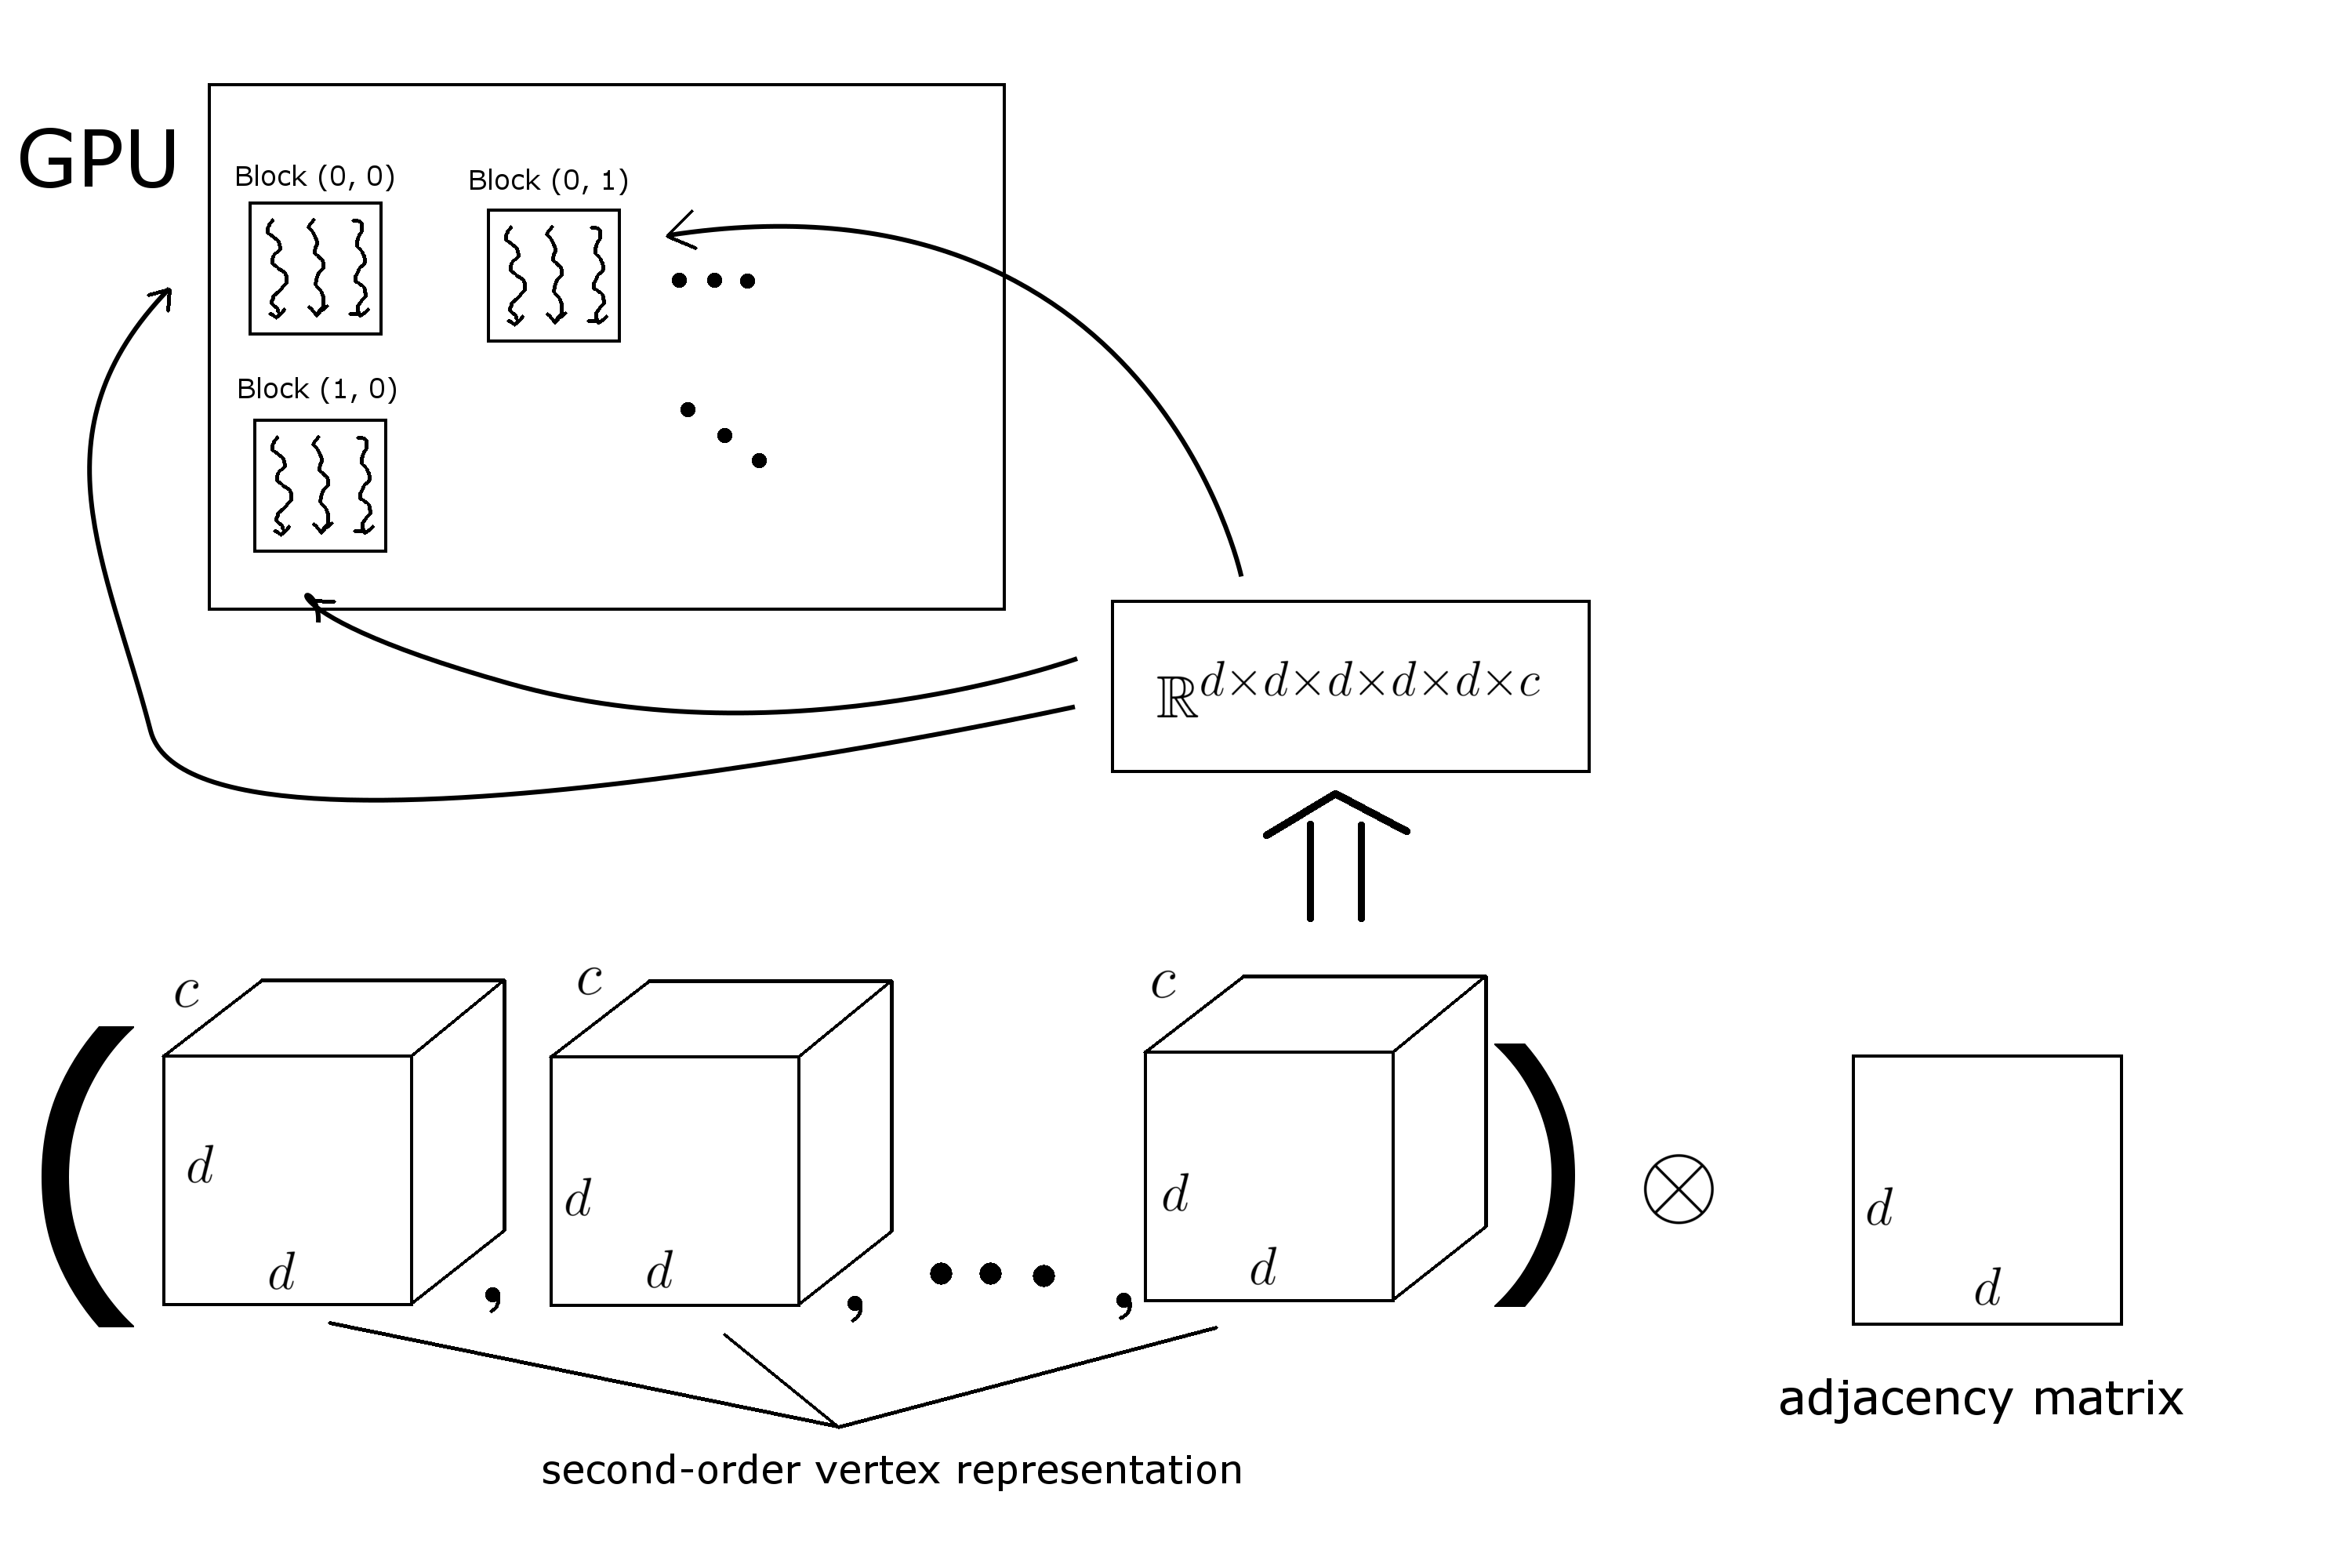
\includegraphics[width=\textwidth]{GPU_multithreading.png}
\end{frame}

\begin{frame}
\frametitle{CPU Multi-threading}
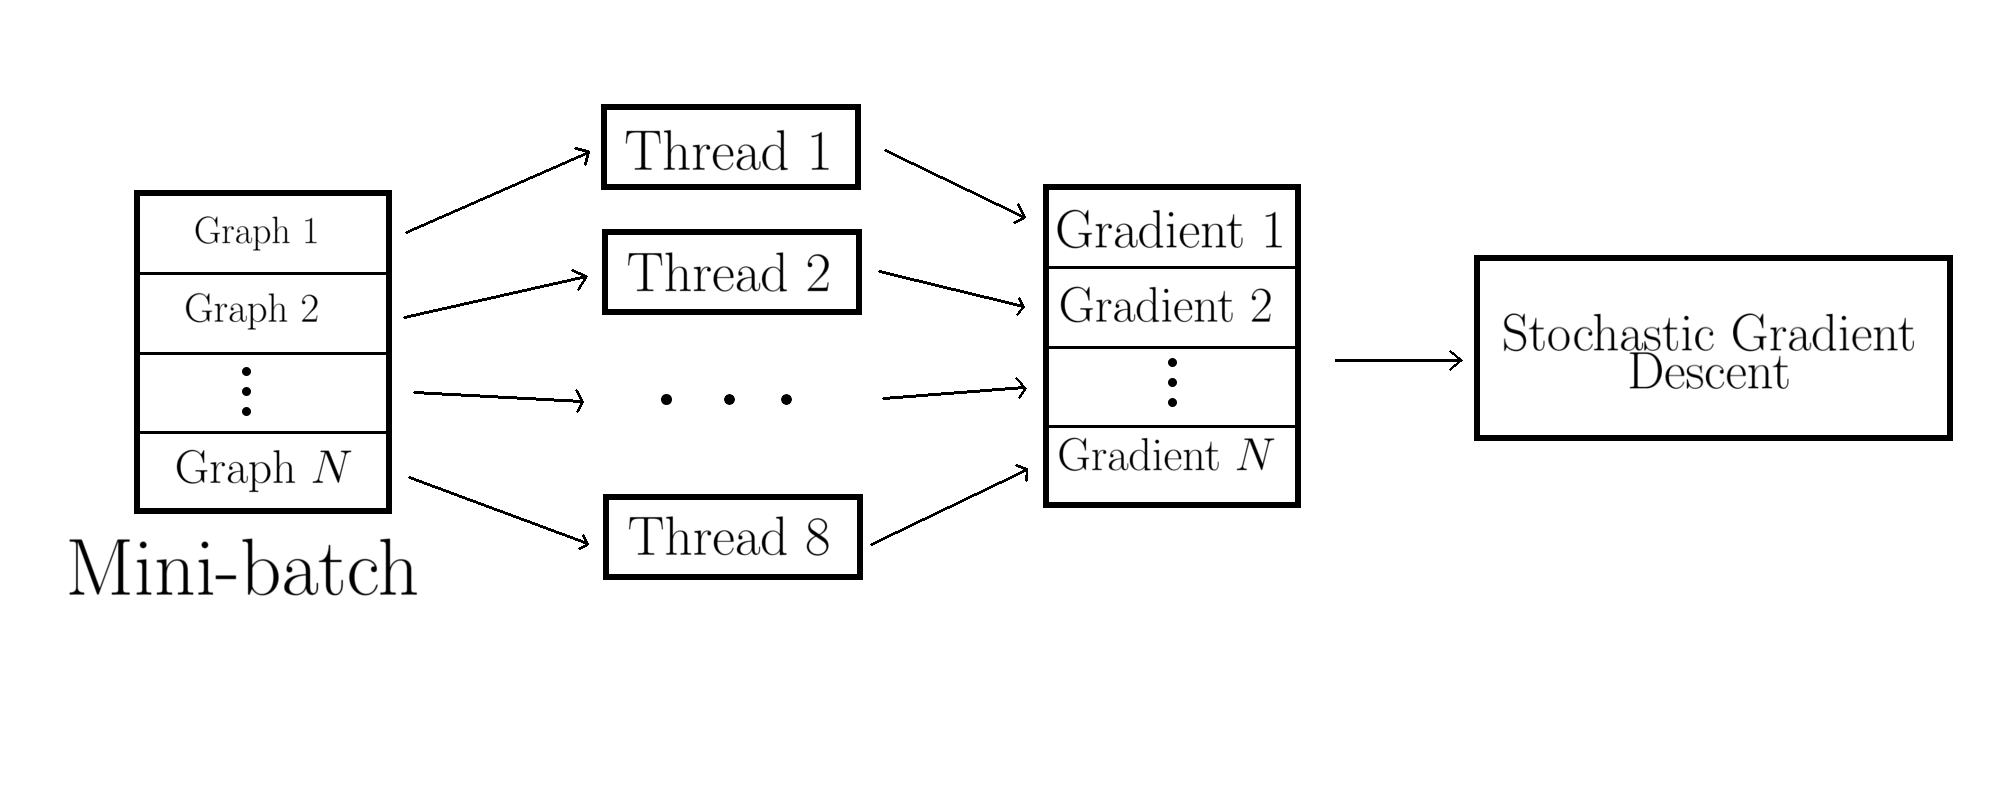
\includegraphics[width=\textwidth]{CPU_multithreading.png}
\end{frame}

\section{Chapter III: Experiments and Results}

\begin{frame}
\frametitle{Performance Test: GPU Matrix Multiplication}
\begin{center}
\begin{tabular}{||c | c | c | c | c ||}
	\hline
	Method & N = 128 & N = 256 & N = 512 & N = 1024 \\
	\hline\hline
	CPU & 22 ms & 379 ms & 2,274 ms & 15,932 ms \\
	\hline
	GPU & < 1 ms & 4 ms & 15 ms & 70 ms \\
	\hline
\end{tabular}
\end{center}
\end{frame}

\begin{frame}
\frametitle{Performance Test: GPU Tensor Contractions}
\begin{center}
\begin{tabular}{|| c | c | c | c | c ||}
	\hline
	$|\Omega_l(v)|$ & $C$ & Floating-points & CPU & GPU \\
	\hline\hline
	5 & 10 & 562,500 & 3 ms & 3 ms \\
	\hline
	5 & 20 & 1,125,000 & 7 ms & 1 ms \\
	\hline
	10 & 10 & 18,000,000 & 56 ms & 1 ms \\
	\hline
	10 & 20 & 36,000,000 & 103 ms & 3 ms \\
	\hline
	20 & 10 & 576,000,000 & 977 ms & 18 ms \\
	\hline 
	20 & 20 & 1,152,000,000 & 2,048 ms & 27 ms \\
	\hline
	35 & 10 & 9,453,937,500 & 12,153 ms & 267 ms \\
	\hline
	35 & 20 & 18,907,875,000 & 25,949 ms & 419 ms \\
	\hline
\end{tabular}
\end{center}
Tensor contraction complexity: $O(18 \times |\Omega_l(v)|^5 \times C)$
\end{frame}

\begin{frame}
\frametitle{Graph Test: Put the whole network together}
\begin{center}
\begin{tabular}{|| c | c | c | c | c | c ||}
	\hline
	$|V|$ & Max $|\Omega_l(v)|$ & $C$ & $L$ & CPU & GPU \\
	\hline\hline
	10 & 10 & 10 & 6 & 1,560 ms & 567 ms \\
	\hline
	15 & 10 & 10 & 6 & 1,664 ms & 543 ms \\
	\hline 
	20 & 15 & 10 & 6 & 7,684 ms & 1,529 ms \\
	\hline
	25 & 15 & 10 & 6 & 11,777 ms & 1,939 ms \\
	\hline
\end{tabular}
\end{center}
\begin{itemize}
	\item $|V|$ is the number of vertices of the input graph
	\item $|\Omega_l(v)|$ is the size of the receptive field
	\item $C$ is the number of channels
	\item $L$ is the number of neural network layers
\end{itemize}
Graphs are generated by Erdos-Renyi random graph model.
\end{frame}

\begin{frame}
\frametitle{Molecular/Graph Test: Small-scale}
\begin{center}
\begin{tabular}{|| c | c | c | c ||}	
	\hline
	Model & Layers & Single-thread & Multi-thread \\
	\hline\hline
	CCN 1D & 1 & 1,836 ms & 874 ms \\
	\hline
	CCN 1D & 2 & 4,142 ms & 1,656 ms\\
	\hline
	CCN 1D & 4 & 9,574 ms & 3,662 ms \\
	\hline
	CCN 1D & 8 (deep) & 20,581 ms & 7,628 ms \\
	\hline
	CCN 1D & 16 (very deep) & 42,532 ms & 15,741 ms\\
	\hline
	CCN 2D & 1 & 35 seconds & 10 seconds \\
	\hline
	CCN 2D & 2 & 161 seconds & 49 seconds \\
	\hline
\end{tabular}
\end{center}
This is the training / testing time on a small dataset of 4 molecules $CH_4$, $NH_3$, $H_20$, $C_2H_4$ with 1,024 epochs (after each epoch, we evaluate the network). All models are fully converged.
\end{frame}

\begin{frame}
\frametitle{Real-world Dataset}
This is what we submitted to ICLR 2018 on October 27, 2017:
\begin{center}
\begin{tabular}{||c | c | c | c | c ||}
	\hline
	Model & Test MAE & Test RMSE \\ 
	\hline
	CCN 1D & 0.532 & 0.773 \\
	\hline
	CCN 2D & 0.570 & 0.773 \\
	\hline
\end{tabular}
\end{center}
This is what we get after the improvement with parallelization (faster models, more epochs can be done):
\begin{center}
\begin{tabular}{||c | c | c | c | c | c ||}
	\hline
	Model & Test MAE & Test RMSE & Percentage of improvement\\ 
	\hline
	CCN 1D & 0.227 & 0.303 & 57.33 \% \\
	\hline
	CCN 2D & 0.343 & 0.458 & 39.82 \% \\
	\hline
\end{tabular}
\end{center}
\end{frame}

\section{Chapter IV: Conclusion and Future Research}

\begin{frame}
\frametitle{Conclusion and Future Research}
\begin{justify}
We implemented the state-of-the-art generalized convolution operation for Graph Neural Networks in order to approximate Density Functional Theory. We obtained very promising results on the Harvard Clean Energy Project dataset.
$$$$
We are developing our custom Deep Learning framework in CUDA/C++, \textbf{GraphFlow}, which supports symbolic differentiation and dynamic computation graph. We expect that this framework will enable us to design more flexible, efficient Graph Neural Networks at a large scale in the future.
\end{justify}
\end{frame}

\begin{frame}
\frametitle{Acknowledgements}
\begin{justify}
We would like to acknowledge Professor Risi Kondor for his valuable instruction and especially for his ideas for generalizing convolution operations in graphs. We also want to thank other members of Machine Learning group at the University of Chicago for their dedicated support.
$$$$
We also want to thank Professor Shan Lu teaching the operating systems course and inspiring this project.
$$$$
Some of the neural network training in this paper was done using the Techstaff cluster of the Department of Computer Science and Midway cluster of the UChicago Computing Research Center.
\end{justify}
\end{frame}

\begin{frame}
\frametitle{Reference}
\begin{justify}
\begin{thebibliography}{9}

\bibitem[1]{Nino}
   N. Shervashidze, P. Schweitzer, E. J. van Leeuwen, K. Mehlhorn, K. M. Borgwardt,
   ``Weisfeiler-Lehman Graph Kernels'',
   \textit{Journal of Machine Learning Research}, vol.~12, 2011.
   
\bibitem[2]{Johannes}
   J. Hachmann, R. O. Amaya, S. A. Evrenk, C. A. Bedolla, R. S. S. Carrera, A. G. Parker, L. Vogt, A. M. Brockway, and A. A. Guzik,
   ``The Harvard Clean Energy Project: Large-Scale Computational Screening and Design of Organic Photovoltaics on the World Community Grid'',
   \textit{The Journal of Physical Chemistry Letters}, pp.~2241--2251, 2011.

\bibitem[3]{Risi}
   R. I. Kondor, and J. Lafferty,
   ``Diffusion Kernels on Graphs and Other Discrete Structures'',
   \textit{International Conference on Machine Learning (ICML)}, 2002.
   
\end{thebibliography}
\end{justify}
\end{frame}

\begin{frame}
\frametitle{Reference}
\begin{justify}
\begin{thebibliography}{9}

\bibitem[4]{Nils}
   N. M. Kriege, P. L. Giscard, R. C. Wilson,
   ``On Valid Optimal Assignment Kernels and Applications to Graph Classification'',
   \textit{Neural Information Processing Systems (NIPS)}, 2016.

\bibitem[5]{Steven}
   S. Kearnes, K. McCloskey, M. Berndl, V. Pande, P. Riley,
   ``Molecular Graph Convolutions: Moving Beyond Fingerprints'',
   \textit{Journal of Computer-Aided Molecular Design}, vol.~30, pp.~595--608, 2016.

\bibitem[6]{Duvenaud}
   D. Duvenaud, D. Maclaurin, J. A. Iparraguirre, R. G. Bombarelli, T. Hirzel, A. A. Guzik, R. P. Adams,
   ``Convolutional Networks on Graphs for Learning Molecular Fingerprints'',
   \textit{Neural Information Processing Systems (NIPS)}, 2015.
  
\end{thebibliography}
\end{justify}
\end{frame}

\begin{frame}
\frametitle{Reference}
\begin{justify}
\begin{thebibliography}{9}
   
\bibitem[7]{Thomas}
   T. N. Kipf, M. Welling,
   ``Semi-Supervised Classification with Graph Convolutional Networks'',
   \textit{International Conference on Learning Representations (ICLR)}, 2017.

\bibitem[8]{Maaten}
   L. V. D. Maaten, G. Hinton,
   ``Visualizing Data using t-SNE'',
   \textit{Journal of Machine Learning Research}, vol.~9, pp.~2579--2605, 2008.

\end{thebibliography}
\end{justify}
\end{frame}

\begin{frame}
\frametitle{}
\begin{center}
Thank you very much for your attention!
\end{center}
\end{frame}


\end{document}